\documentclass[12pt]{report}

\renewcommand{\familydefault}{\sfdefault} % San Serif Font

\usepackage[margin=1in]{geometry}
\usepackage{graphicx}
\usepackage{hyperref}
\usepackage{placeins}
\usepackage{textcomp}
\usepackage{wrapfig}

\newcommand{\imageright}[3]{
    \begin{wrapfigure}{r}{#2\textwidth}
        \centering
        \includegraphics[width=#2\textwidth]{#1}
        \vspace*{#3}
    \end{wrapfigure}
}

\begin{document}
\raggedright

\title{3D Printing Guide}
\chapter*{3D Printing Guide}

\section*{Print Preperation}
\label{sec:preperation}

\subsection*{Exporting from Fusion 360}
\label{sec:exporting}

\imageright{export_body.png}{0.5}{-2cm}

To export a model from Fusion 360 for printing, follow the following steps.

\begin{itemize}
    \item Ensure the part that you wish to print is a single \textit{body} in
        Fusion 360. You may need to select multiple bodies and use the
        \textit{Combine} tool to unify them.
    \item Navigating to \textit{Bodies} in the object browser in the top left,
        find the body you wish to print. Right click on it and select
        \textit{Save as Mesh}. Choose \texttt{STL} as the format,
        \textit{Binary} or \textit{ASCII} will both work fine. 
\end{itemize}

You can use this 3D model file for slicing in Cura, or other slicing software.

\pagebreak
\subsection*{Setting Up Cura}
\label{sec:setup}

The slicing software we recommend is Ultimaker Cura, which you can download by
searching for Cura and downloading the first result. \par
The screenshots used in this guide come from version 4.13, but more recent
versions or slightly older versions should be similar. \par
When installing Cura you may be prompted to install various Adafruit and
Arduino drivers. These are optional but you may as well install them as you'll
likely need them if you plan to work with Arduino later on. \par
Once you've installed the application, when you launch it for the first time,
various prompts will appear with information about the version of Cura you've
installed, etc. None of these matter except for the one which asks that you
add a printer. \par
During this step, you should select \textit{Add a non-networked printer} and
navigate to choose either a Creality Ender 3 or a Prusa3D i3 MK3S, as these
are the two printers we have (at time of writing). You can easily add more
printers at a later date, so it doesn't matter very much which you choose.

\begin{center}
    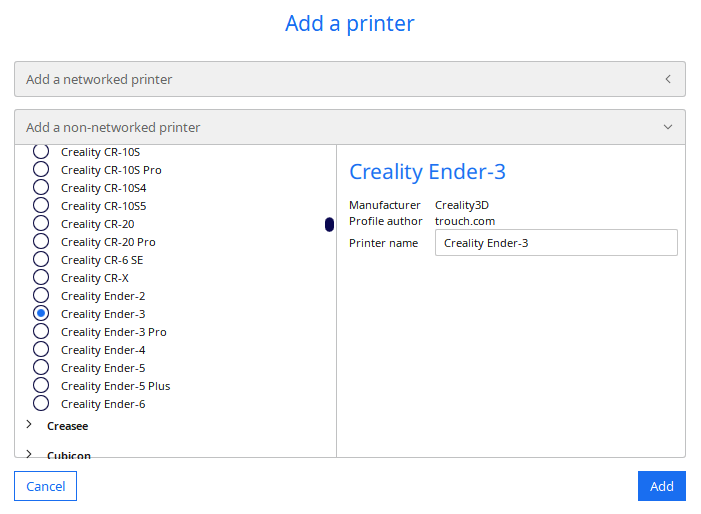
\includegraphics[width=0.6\textwidth]{add_printer.png}
    \vspace*{-2cm}
\end{center}

\pagebreak

{

\subsection*{Slicing In Cura}
\label{sec:slicing}

\imageright{slicing_settings.png}{0.25}{-1cm}

Launch Cura and select the folder icon in the top left corner to load your 3D
model (repeat this process if you want to print multiple models). \par
Make sure you have the appropriate 3D printer selected for your current print
job. Click the material settings tab in the middle and ensure that
\textit{Generic PLA} is selected, with the appropriate nozzle diameter for the
printer you're slicing for. \par
Open the settings menu in the top right corner and configure the following
settings appropriately. To find them you might need to click \textit{Custom} and
then use the search bar. It may take you a little while to develop an intuition
for what a given print will require, but the defaults specified below should
generally work well.

}

\begin{itemize}
    \item \textit{Layer Height} dictates how thick each layer of the print will
        be. This should generally be set to around half the
        nozzle diameter. For the default 0.4mm nozzle, this means a layer height
        of 0.2mm is a good choice. You may want to use a lower layer height for
        parts where good detail is important, though this will result in longer
        print times.
    \item \textit{Line Width} should generally be set to 120\% of the nozzle
        diameter. So for a 0.4mm nozzle, this would be 0.48mm.
    \item \textit{Infill Density} refers to the proportion of the interior of
        the print which is solid plastic; below 100\%, the print will have a
        pattern printed inside rather than being solid, and this is desireable
        because it speeds up prints and reduces material usage, generally
        without much loss in strength. \textit{Infill Density} should be set
        to somewhere around 10-20\% for draft parts or parts which won't be
        subjected to significant strain, or 40-50\% for final parts which are
        under strain. Beyond 50\%, increases in infill density provide minimal
        benefit to the strength of parts.
    \item \textit{Build Plate Adhesion Type} refers to the type of pre-part
        structure used to get the material sticking to the bed. Generally, you
        can safely set this to \textit{None}, however, particularly on lower end
        machines, like our Ender 3, it can be useful to use a skirt or brim.
        These are thin outlines layed down around the part, to improve the
        chances of good early layers. For extremely delicate parts, one might
        consider using the \textit{Raft} setting which causes the printer to lay
        down a small bed of material under the printed part.
    \item \textit{Generate Support} should be set to true if your part has
        significant overhangs. For parts with arches or other considered
        bridges, suppot can often be avoided, but parts with right angle
        overhangs should almost always be printed with support.
    \item \textit{Suppot Overhang Angle} refers to the minimum angle a part of
        the model must overhang by before a support tower will be generated at
        that location. Cura defaults to a very conservative 45\textdegree angle
        for this, but you can usually set it much higher, to around
        65-70\textdegree. This will mean less support is generated so less will
        need to be removed and you may have a cleaner model. This setting can be
        ignored if your model doesn't need supports.
\end{itemize}

Feel free to try out other settings if you feel they are relevant to your print
(or could be fun!). Once you're happy with your configuration, press
\textit{Slice} to generate the \texttt{gcode} file for the printer. \par
Once you've sliced your model, you can click \textit{Preview} at the top center
of the screen to access a layer-by-layer overview of the print. You'll be able
to see the generated supports, bed adhesion and other helpers here. If this
looks good, save the file by clicking \textit{Save to Disk} (or save directly
to a micro SD card for printing).

\pagebreak
\section*{Printers}
\label{sec:printers}

We presently (as of March 2022) have two 3D printers at Robotics Club. These are
are a Creality Ender 3 and a Prusa3D i3 MK3S. Make sure that you use the right
profile when printing, as it will affect the available print area and print head
dimensions, which must be correct for a successful print.

\subsection*{Bed Levelling}
\label{sec:levelling}

Before printing, the bed of a 3D Printer must be levelled to ensure a flat
surface for the model to be layed on. The Prusa printer has \textit{automatic
bed levelling}, so no extra step needs to be taken if you are using this
printer. It will instead automatically move the head across the print bed and
test the bed height at a matrix of positions, which it uses to perform software
adjustments without your input. The Ender requires manual bed levelling, which
is a little more involved. The process is as follows

\begin{itemize}
    \item Turn on the printer, and press the wheel on the front panel to access
        the menu. Using the wheel, navigate to \texttt{Control > Temperature >
        Bed} and set it to something warm but not dangerous, around 40 or 50
        \textdegree C. Ensure the nozzle temperature is set to 0. Let the
        print bed warm, as it will warp slightly as it does so. You can see the
        temperature on the home screen.
    \item Select \texttt{Prepare > Auto Home} and press to confirm. The print
        head will navigate to the front left corner of the print bed. Select
        \texttt{Prepare > Disable Steppers} to disable the motors so you can
        slide around the bed and print head.
    \item Take a piece of paper (printer paper works perfectly) and slide it
        between the nozzle and the print bed. If you can't, you may need to turn
        the wheel on the underside of the print bed counter-clockwise to
        increase the gap between the print bed and nozzle.
    \item Test how tight the nozzle is against the sheet of paper. You should be
        able to move the paper without tearing it, but should still feel some
        friction with the nozzle. Using the wheel below the print bed, turning
        clockwise to loosen the nozzle and vice versa to tighten, adjust the
        nozzle to this tightness.
    \item Sliding the nozzle left-to-right and the bed front-to-back, repeat
        this process for the other three corners of the print bed, such that
        the nozzle has the same light friction with the nozzle in each corner.
        Make sure you re-test the corners you've done once you finish, as
        adjusting one corner may affect the tightness of another.
   \item Once you're satisfied that the nozzle is at roughly the height of a
        sheet of paper in all four corners of the print bed, the bed is level.
        Congratulations!
\end{itemize}

\pagebreak
\subsection*{Printing}
\label{sec:printing}

To 3D print a file, first \hyperref[sec:slicing]{slice it}, making sure that you
select the printer you are using and that you choose the correct nozzle size (at
time of writing we are using a 0.8mm nozzle on the Ender and a 0.4mm nozzle on
the Prusa, but you should check on the printer or confirm with a mentor as this
is subject to change). \par
When slicing, you will produce a \texttt{.gcode} file, which you can either save
to a micro SD card directly through Cura or copy across. If you don't have a
micro SD card slot, micro SD to SD adapters are available (ask a mentor), or
send your file to a peer who does and get them to save it for you. \par
Once you have your file on a micro SD card, you can take it to the printer to
print. See the individual printing instructions for each printer below. 

\imageright{ender.jpg}{.25}{-2cm}
\subsubsection*{Ender}

\begin{itemize}
    \item Make sure that you \hyperref[sec:levelling]{level the bed} before
        printing.
    \item Plug the micro SD card into the slot at the front bottom of the
        printer.
    \item If the printer hasn't registered the SD card yet, select
        \texttt{Init. SD card} to do so.
    \item Select \texttt{Print from SD} and then the file you wish to
        print. The printer should begin heating and start printing once fully
        hot. Don't touch the nozzle or print bed while they're hot.
    \item If you notice something going wrong during the print, select
        \texttt{Stop print} to abort.
\end{itemize}

\imageright{prusa.jpg}{.25}{-2cm}
\subsubsection*{Prusa}

\begin{itemize}
    \item Place the micro SD card in a micro SD to SD card adapter (there may
        already be one in the slot on the left side of the printer's front
        panel).
    \item Plug the SD card into the slot on the left of the printer's front
        panel. The printer should detect it automatically.
    \item Press the knob and scroll to \texttt{Print from SD}. Select the file
        you wish to print and press to confirm. The printer should heat up and
        then begin the automatic bed levelling process, before beginning to
        print.
    \item If you notice something going wrong during the print, select
        \texttt{Stop print} to abort.
\end{itemize}

\end{document}
